%   Titre de la sous sections
\section{Mon titre génial avec \mb}

%   logo mb ou st dans la table des matières
\logo{mb}
%\logo{mbot}
%\logo{st}

%
%   style de la page
%   commenter avec % le style non utilisé
\pagestyle{mb} %pour microbit
%\pagestyle{mbot} %pour mbot
%\pagestyle{st} %pour ST

\subsection{Description}

\subsubsection{Objectif}


%   bloc de formule
%   sans titre et fond bleu cyan
\begin{formule}
Le but de ce projet\ldots
\end{formule}


\subsubsection{Intérêt}

L'intérêt de traiter ce projet avec\ldots

%liste d'arguments
\begin{description}
    \item [1er argument] détail
    \item [2ème argument] détail
    \item [2ème argument] détail
\end{description}


\subsubsection{Matériel}
\begin{itemize}
%   matériel pour micro:bit
    \item 1 $\times$ \matosMb \emph{(facultatif car le simulateur peut suffire)}
%   site pour micro:bit
    \item 1 $\times$ accès internet : IDE programmation par bloc \url{http://makecode.microbit.org/}
%   matériel pour ST
    \item 1 $\times$ \matosSt \emph{(facultatif car le simulateur peut suffire)}
%   site internet pour ST
   \item 1 $\times$ accès internet : IDE programmation par bloc \url{https://makecode.st.com/}
%   matériel pour MBot
    \item 1 $\times$ \matosMbot
%   site internet pour MBot
   \item 1 $\times$ accès internet : IDE programmation par bloc \url{http://editor.makeblock.com/ide.html}
\end{itemize}



\subsubsection{Remarques}


%   bloc méthode
%   titre + fond bleu
\begin{methode}
    Quelques détails
    \ldots % points de suspensions
    
    \begin{enumerate}
        \item \textbf{Initiation - Premier modèle.} \\
            bla bla\ldots % points de suspensions
        \item \textbf{Intermédiaire - Pile ou Face.}\\
            bla bla\ldots % points de suspensions
    \end{enumerate}
\end{methode}

%
% activité de niveau 
%

%   saut de page
\newpage

%   titre de la sous section
\subsection{Niveau initiation - \ldots}

\subsubsection{Activité élève}

% commande perso \CARTOUCHE
%   5 paramètres : 
%       * durée
%       * public
%       * travail en maths
%       * travail en sciences
%       * travail en algo
\cartouche
{0,5 h}         %durée
{2de}           %public
{calcul}        %maths
{mouvement}     %sciences
{boucles}       %algo


%   petite image de logo qui va
%   se mettre dans le bloc élève
\begin{wrapfigure}[4]{r}{3cm}
    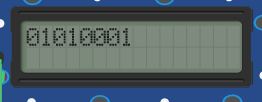
\includegraphics[width=\linewidth]{res/st-pf-00.png}
\end{wrapfigure}

%   bloc élève
%   fond orange
\begin{eleve}    
    \texttt{\textsc{Ta Mission} : Utiliser\ldots avec \emph{énergie}!}
    
%   ajout d'une image
    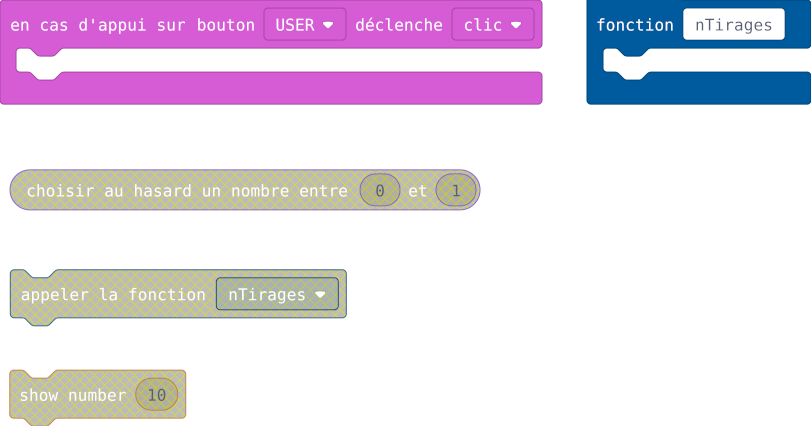
\includegraphics[width=0.5\linewidth]{res/st-pf-00-eleve.png}
\end{eleve}



\subsubsection{Notes pour l'enseignant}

%
%   méthode et remarque
%
\begin{methode}
Proposition de résolution :

bla bla\ldots
\end{methode}


\begin{remarque}
    La proposition de solution \emph{interactive} est accessible en ligne \url{https://makecode.com/_EMYM0YfT11A6}.
\end{remarque}


%
%   méthode et remarque V2
%   version sur 2 colonnes
%   pour cela utiliser l'environnement minipage

%   colonne de gauche
\begin{minipage}[t]{0.7\linewidth}
    \begin{methode}~\\
    Proposition de résolution :
    
    bla bla\ldots
    \end{methode}
\end{minipage}
%   petit "ressort"
%   pour centrer les 2 colonnes
\hfill
%   colonne de droite
\begin{minipage}[t]{0.3\linewidth}
    \begin{remarque}~\\
        La proposition de solution \emph{interactive} est accessible en ligne \url{https://makecode.com/_EMYM0YfT11A6}.
    \end{remarque}
\end{minipage}